\section{Matrix Based CFPQ for Single-Path Semantics}
In this section, we propose the matrix-based algorithm for CFPQ w.r.t. the single-path query semantics (see listing~\ref{lst:algo2}). This algorithm constructs the set of matrices $T$ with PathIndexes as elements.
{\small
	\begin{algorithm}
		\floatname{algorithm}{Listing}
		\begin{algorithmic}[1]
			\caption{CFPQ algorithm w.r.t. single-path query semantics}
			\label{lst:algo2}
			\Function{evalCFPQ}{$D=(V,E), G=(N,\Sigma,P)$}
			\State{$n \gets$ |V|}
			\State{$T \gets \{T^{A_i} \mid A_i \in N, T^{A_i}$ is a matrix $n \times n$, $T^{A_i}_{k,l} \gets \bot$ \} }
			\ForAll{$(i,x,j) \in E$, $A_k \mid A_k \to x \in P$}
			%\Comment{Matrices initialization}
			%\For{$A_k \mid A_k \to x \in P$}
			{$T^{A_k}_{i,j} \gets (i,j,i,1,1)$}
			%\EndFor
			\EndFor
			\For{$A_k \mid A_k \to \varepsilon \in P$}
			{$T^{A_k}_{i,i} \gets (i,i,i,1,0)$}
			\EndFor
			
			\While{any matrix in $T$ is changing}
			%\Comment{Transitive closure calculation}
			\For{$A_i \to A_j A_k \in P$}
			{ $T^{A_i} \gets T^{A_i} + (T^{A_j} \odot T^{A_k})$ } 
			\EndFor
			\EndWhile
			\State \Return $T$
			\EndFunction
		\end{algorithmic}
	\end{algorithm}
}

After constructing the set of matrices $T$ for every node pair $i, j$ and nonterminal $A$ we can extract a path $i \pi j$ from $i$ to $j$ such that $A \xRightarrow[G]{*} l(\pi)$ if such path exists. We also propose the algorithm (see listing~\ref{lst:algo3}) for extracting one of those paths which forms a string with minimal height of derivation tree. Our algorithm returns the empty path $[]$ only if $i = j$ and $A \to \varepsilon \in P$. Note that if the PathIndex for given $i,j,A$ is equal to $\bot$ then our algorithm returns a special path $\pi_{\emptyset}$ to denote that such a path does not exist.

{\small
	\begin{algorithm}
		\floatname{algorithm}{Listing}
		\begin{algorithmic}[1]
			\caption{Path extraction algorithm}
			\label{lst:algo3}
			\Function{extractPath}{$i, j, A, T=\{T^{A_i}\}, G=(N,\Sigma,P)$}
			\State{$index \gets T^{A}_{i,j}$ }
			
			\If{$index = \bot$}
			\State \Return $\pi_{\emptyset}$
			\Comment{Such a path does not exist}
			\EndIf
			
			\If{$index.height = 1$}
			\If{$index.length = 0$}
			\State \Return $[]$
			\Comment{Return an empty path}
			\EndIf
			\ForAll{$ x \mid (i,x,j) \in E$}
			\If{$A \to x \in P$}
			\State \Return $[(i,x,j)]$
			\Comment{Return a path of length one}
			\EndIf
			\EndFor
			\EndIf
			
			\ForAll{$A \to B C \in P$}
			\State{$index_B \gets T^{B}_{i,index.middle}$ }
			\State{$index_C \gets T^{C}_{index.middle,j}$ }			
			\If{$(index_B \neq \bot) \wedge (index_C \neq \bot)$}
			\State{$maxH \gets max(index_B.height, index_C.height)$ }
			\If{$index.height = maxH + 1$}
			
						
			\State{$\pi_1 \gets$ \Call{extractPath}{$i, index.middle, B, T, G$}}
			\State{$\pi_2 \gets$ \Call{extractPath}{$index.middle, j, C, T, G$}}
			\State \Return $\pi_1 + \pi_2$
			\EndIf
			\EndIf
			\EndFor
			\EndFunction
		\end{algorithmic}
	\end{algorithm}
}

\subsection{Correctness}

Let $T^{(p)} = \{T^{(p), A_i}\}$ be a constructed matrix $T$ by the algorithm in listing~\ref{lst:algo2} after $p-1$ loop iterations for $p \geq 2$, and $T^{(1)} = \{T^{(1), A_i}\}$ be a constructed matrix $T$ by this algorithm after initialization in lines 3-5. Note that the matrix $T$ returned by this algorithm is equal to $\sum_{p = 1}^{\infty} T^{(p)}$. Then the following lemma and theorem hold.

\begin{lemma}\label{lemma:correctness}
	Let $D = (V,E)$ be a graph, let $G =(N,\Sigma,P)$ be a grammar. Then for any $i, j$ and for any non-terminal $A \in N$, $index = T^{(p),A}_{i,j}$ and $index = (i,j,k,h,l) \neq \bot$ iff $(i,j) \in R_A$ and $i \pi j$, such that there is a derivation tree of the minimal height $h \leq p$ for the string $l(\pi)$  of length $l$ and a context-free grammar $G_A = (N,\Sigma,P,A)$.
\end{lemma}
\begin{proof}(Proof by Induction)
	
	\textbf{Base case}: Show that the lemma holds for $p = 1$. For any $i, j$ and for any non-terminal $A \in N$, $(i,j,k,h,l) = T^{(1), A}_{i,j}$ iff there is either $i \pi j$ of length $1$ that consists of a unique edge $e$ from the node $i$ to the node $j$ and $(A \rightarrow x) \in P$, where $x = l(\pi)$, or $i = j$ and $(A \rightarrow \varepsilon) \in P$, where $\varepsilon = l(\pi)$. Therefore $(i,j) \in R_A$ and there is a derivation tree of the minimal height $h = p = 1$, shown on Figure~\ref{tree1}, for the string $x$ and a context-free grammar $G_A = (N,\Sigma,P,A)$. Thus, it has been shown that the lemma holds for $p = 1$.
	
	\begin{figure}[h!]
		\centering
		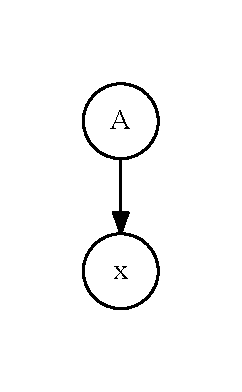
\includegraphics[width=2cm]{pictures/tree1.pdf}
		\caption{The derivation tree of the minimal height $p = 1$ for the string $x = l(\pi)$ where $x \in \Sigma \cup \{\varepsilon\}$.}
		\label{tree1}
	\end{figure}
	
	\textbf{Inductive step}: Assume that the lemma holds for any $p \leq (q - 1)$ and show that it also holds for $p = q$, where $q \geq 2$.
	
	The index $(i,j,k,h,l) = T^{(q),A}_{i,j}$ iff there is exists a rule $(A \to B C) \in P$ such that $(i,j,k,h,l) = M_{i,j}$ where $M = T^{(q-1),A} + (T^{(q-1),B} \odot T^{(q-1),C})$. 
	
	Let $(i,j,k,h,l) = T^{(q-1),A}_{i,j}$. By the inductive hypothesis, $(i,j,k,h,l) = T^{(q-1),A}_{i,j}$ iff $(i,j) \in R_A$ and there exists $i \pi j$, such that there is a derivation tree of the minimal height $h \leq (q-1)$ for the string $l(\pi)$ and a context-free grammar $G_A = (N,\Sigma,P,A)$. The statement of the lemma holds for $p = q$ since the height $h$ of this tree is also less than or equal to $q$.
	
	Now, let $(i,j,k,h,l) = (T^{(q-1),B} \odot T^{(q-1),C})_{i,j}$. By the definition of the binary operation $\odot$, $(i,j,k,h,l) = (T^{(q-1),B} \odot T^{(q-1),C})_{i,j}$ iff there are $r=k$, $(i,r,\_,h_1,l_1) = T^{(q-1),B}_{i,r}$ and $(r,j,\_,h_2,l_2) = T^{(q-1),C}_{r,j}$, such that $q = max(h_1, h_2) + 1$, $l = l_1 + l_2$. Hence, by the inductive hypothesis, there are $i \pi_1 r$ and $r \pi_2 j$, such that $(i,r) \in R_B$ and $(r,j) \in R_C$, and there are the derivation trees $T_B$ and $T_C$ of minimal heights $h_1 \leq (q-1)$ and $h_2 \leq (p-1)$ for the strings $w_1 = l(\pi_1)$, $w_2 = l(\pi_2)$ and the context-free grammars $G_B$, $G_C$ respectively. Thus, the concatenation of paths $\pi_1$ and $\pi_2$ is $i \pi j$, where $(i,j) \in R_A$ and there is a derivation tree of the minimal height $h = 1 + max(h_1, h_2)$, shown on Figure~\ref{tree2}, for the string $w = l(\pi)$ of length $l = l_1 + l_2$ and a context-free grammar $G_A$.
	\begin{figure}[h!]
		\centering
		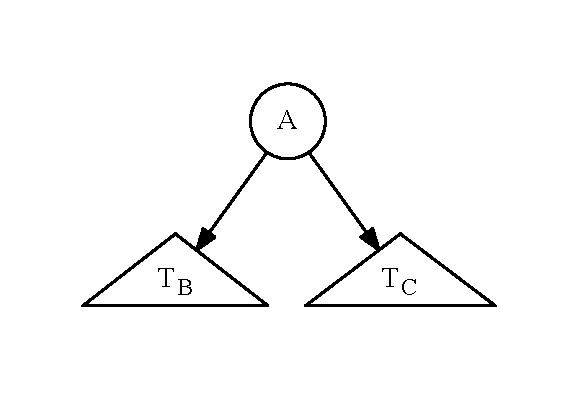
\includegraphics[width=5cm]{pictures/tree2.pdf}
		\caption{The derivation tree of the minimal height $h = 1 + max(h_1, h_2)$ for the string $w = l(\pi)$, where $T_B$ and $T_C$ are the derivation trees for strings $w_1$ and $w_2$ respectively.}
		\label{tree2}
	\end{figure}
	
	The statement of the lemma holds for $p = q$ since the minimal height $h = 1 + max(h_1, h_2) \leq q$. This completes the proof of the lemma.
\end{proof}

\begin{mytheorem}\label{thm:correct}
	Let $D = (V,E)$ be a graph and let $G =(N,\Sigma,P)$ be a grammar. Then for any $i, j$ and for any non-terminal $A \in N$, $index = T^A_{i,j}$ and $index = (i,j,k,h,l) \neq \bot$ iff $(i,j) \in R_A$ and $i \pi j$, such that there is a derivation tree of the minimal height $h$ for the string $l(\pi)$ of length $l$ and a context-free grammar $G_A = (N,\Sigma,P,A)$.
\end{mytheorem}
\begin{proof}
	
	Since the matrix $T = \sum_{p = 1}^{\infty} T^{(p)}$ for any $i, j$ and for any non-terminal $A \in N$, $index = T^A_{i,j}$ and $index = (i,j,k,h,l) \neq \bot$ iff there is $p \geq 1$, such that $index \in T^{(p),A}_{i,j}$. By the lemma~\ref{lemma:correctness}, $index = T^{(p),A}_{i,j}$ iff $(i,j) \in R_A$ and $i \pi j$, such that there is a derivation tree of the minimal height $h \leq p$ for the string $l(\pi)$  of length $l$ and a context-free grammar $G_A = (N,\Sigma,P,A)$. This completes the proof of the theorem.
\end{proof}

We can, therefore, determine whether $(i,j) \in R_A$ by asking whether $\bot = T^A_{i,j}$. Also, we can extract such a path which forms a string with a derivation tree of minimal height by using our algorithm in listing~\ref{lst:algo2}. Thus, we show how the context-free path query evaluation w.r.t. the single-path semantics can be solved in terms of matrix operations.

Correctness of path extraction algorithm?

\subsection{Complexity}
Complexity analysis.

\subsection{Example?}
Example